% t. schneider

%!TEX TS-program = xelatex
%!TEX encoding = UTF-8 Unicode

\documentclass[11pt, letterpaper, oneside]{memoir}
\listfiles
\usepackage{fontspec} 

% FONTS
\defaultfontfeatures{Mapping=tex-text} % converts LaTeX specials (``quotes'' --- dashes etc.) to unicode
\setromanfont{Gentium Plus}
\setverbatimfont{\normalfont\ttfamily\footnotesize}

% HEADINGS
\usepackage{float}
\usepackage{graphicx} 
\graphicspath{{../images/}}
\usepackage[normalem]{ulem} 
\usepackage{threeparttable}
\usepackage[cmex10]{amsmath}
\usepackage{color}
\usepackage[font=footnotesize]{subfig}
\definecolor{goby_orange}{RGB}{227,96,52}
\renewcommand{\colorchapnum}{\color{goby_orange}}
\renewcommand{\colorchaptitle}{\color{goby_orange}}
\definecolor{goby_aqua}{RGB}{28,159,203}
\definecolor{goby_aqua_darkened}{RGB}{14,77,94}


% PDF SETUP
\usepackage[dvipdfm, bookmarks, colorlinks, pdftitle={Goby User Manual},pdfauthor={Goby Developers}]{hyperref} 
\hypersetup{linkcolor=goby_aqua_darkened,citecolor=goby_aqua_darkened,filecolor=black,urlcolor=goby_aqua_darkened} 
\newcommand{\xmltag}[1]{\texttt{$<$#1$>$}}

\setsecnumdepth{subsection}

% GLOSSARIES
\usepackage[toc]{glossaries} % acronym will go in main glossary

\renewcommand{\glsnamefont}[1]{\textit{#1}}

\makeglossaries
\newglossaryentry{acoustic networking}{name={acoustic networking},description={a way of connecting underwater vehicles and other nodes wirelessly using sound waves (since light is rapidly attenuated in sea water). See also \url{http://gobysoft.com/doc/acomms}}}
\newglossaryentry{application}{name={application},description={a collection of code that compiles to a single exectuable unit on your operating system. synonymously (and more precise): processes or binaries}}
\newglossaryentry{pubsub}{name={publish/subscribe},description={a method of communication between processes that is roughly analogous to authors and customers of a newspaper or newsletter. Certain people (applications) publish stories (data) that other people (applications) subscribe for and read in the newsletter. Typically applications perform both tasks, subscribing for some data and publishing others. See also \url{http://en.wikipedia.org/wiki/Publish/subscribe}}}
\newglossaryentry{autonomy architecture}{name={autonomy architecture},description={lossly defined, a collection of software applications and libraries that facilitate communications, decision making, timing, and other utilties needed for making robots function. Another common term for this is autonomy ``middleware''}}
\newglossaryentry{daemon}{name={daemon},description={an application on a Linux/UNIX machine that runs continuously in the background. the \texttt{gobyd} is a server and the Goby applications are clients.}}
\newglossaryentry{star topology}{name={star topology},description={all communications pass through a central mediator (in this case, \texttt{gobyd}) and not directly from any Goby application to another}}
\newacronym[description={a language (in the sense of a programming language) that allows querying or accessing data from a database. For example, if I wanted to know the best baseball players in history and I had a database of players' stats, I could write in SQL the following query that would provide the data I need: \texttt{"SELECT * FROM baseball\_players WHERE batting\_average > 0.300 ORDER BY batting\_average DESC"}}]{sql}{SQL}{Structured Query Language}
\newacronym[description={From \cite{protobuf}: ``Protocol buffers are Google's language-neutral, platform-neutral, extensible mechanism for serializing structured data – think XML, but smaller, faster, and simpler. You define how you want your data to be structured once, then you can use special generated source code to easily write and read your structured data to and from a variety of data streams and using a variety of languages – Java, C++, or Python.''}]{protobuf}{protobuf}{Google Protocol Buffers}
\newglossaryentry{base class}{name={base class},plural={base classes},description={also known as subclass or child class}}
\newglossaryentry{derived class}{name={derived class},plural={derived classes},description={also known as superclass or parent class}}
\newglossaryentry{virtual}{name={virtual},description={A member of a \gls{base class} than can be redefined in a \gls{derived class}. See also \url{http://www.cplusplus.com/doc/tutorial/polymorphism/}}}
\newglossaryentry{synchronous}{name={synchronous},description={From \cite{mw-synchronous}: "recurring or operating at exactly the same period."}}
\newglossaryentry{asynchronous}{name={asynchronous},description={From \cite{mw-asynchronous}: " of, used in, or being digital communication (as between computers) in which there is no timing requirement for transmission and in which the start of each character is individually signaled by the transmitting device."}}
\newacronym[description={A multidiscplinary research group at the Center for Ocean Engineering (Dept. of Mechanical Engineering) at Massachusetts Institute of Technology. LAMSS focuses on collaborative marine robotics for a variety of acoustic and non acoustic sensing tasks. See \url{http://lamss.mit.edu}.}]{lamss}{LAMSS}{Laboratory for Autonomous Marine Sensing Systems}


% DOCUMENT

\begin{document}

\begin{center}
\begin{Large}
Goby Underwater Autonomy Project\\
\vspace{0.5em}
\includegraphics[height=3em]{gobysoft_logo_image_only.eps} \\
\vspace{0.5em}
\end{Large}
\begin{LARGE}
User Manual for Version 1.0\\
\vspace{0.5em}
\end{LARGE}
<\url{https://launchpad.net/goby}>



\end{center}
\vspace{0.5em}
\rule{\textwidth}{1pt}

\vspace{0.5em}

\tableofcontents

%\wrappingon
\linenumberfrequency{1}
\bvnumbersoutside
\linenumberfont{\normalfont\tiny}
\chapterstyle{pedersen}
\setsecheadstyle{\Large\raggedright}
\setsubsecheadstyle{\large\raggedright}
\setsubsubsecheadstyle{\itshape\raggedright}
\setparaheadstyle{\itshape\raggedright}
\setsubparaheadstyle{\itshape\raggedright}

\hangsecnum

\chapter{Introduction}

\section{What is Goby?}

The Goby Underwater Autonomy Project is an \gls{autonomy architecture} tailored for marine robotics with a focus on intervehicle communication.

Currently, Goby has three major parts:

\begin{itemize}
\item Goby-Acomms: The Goby Acoustic Communications library (\verb|goby-acomms|) has been provided since Version 1.0. See the Developers' documentation for details on these library and the various modules it contains at \cite{goby-doc}. Users of the MOOS application \verb|pAcommsHandler| should see Chapter \ref{chap:MOOS}.
\item Goby-Util: A utility library that provide functions for dealing with time, type conversion, binary conversions, etc. This library is intended to be small, as Goby makes use of the C++ Standard Library and Boost for most utility tasks.
\item Goby-Core: An \gls{autonomy architecture} that ties together various marshalling schemes (Google Protocol Buffers, MOOS, LCM, etc.) and provides a message passing middleware based on ZeroMQ (for ethernet) and Goby-DCCL (for acoustic communications). Goby-Core will be provided in release version 3.0.
\end{itemize}

\section{Structure of this Manual}
This manual covers the MOOS Applications that use Goby-Acomms release version 2.0. If you are interested in the C++ Goby-Acomms libraries directly, please read the online Developers' documentation at \cite{goby-doc} In fact, you may want to go download and install Goby now before reading further: \url{https://launchpad.net/goby}.

\section{How to get help}
The Goby community is here to support you. This is an open source project so we have limited time and resources, but you will find that many are willing to contribute their help, with the hope that you will do the same as you gain experience. Please consult these resources and people, probably in this order of preference:

\begin{enumerate}
\item This user manual. % TODO(tes) put in link this manual
\item The Wiki: \url{http://gobysoft.com/wiki}.
\item Questions and Answers on Launchpad: \url{https://answers.launchpad.net/goby}.
\item The developers' documentation: \url{http://gobysoft.com/doc}.
\item Email the listserver \href{mailto:goby@mit.edu}{goby@mit.edu}. Please sign up first: \url{http://mailman.mit.edu/mailman/listinfo/goby}.
\item Email the lead developer (T. Schneider): \href{mailto:tes@mit.edu}{tes@mit.edu}.
\end{enumerate}


\chapter{The Hello World example}
\epigraph{\textit{``It's a dangerous business, Frodo, going out of your door,'' he used to say. ``You step into the Road, and if you don't keep your feet, there is no knowing where you might be swept off to.''}}{J.R.R. Tolkien, \textit{The Fellowship of the Ring} (1954)}



\MakeShortVerb{\!} % makes \verb|foo| == !foo!

Goby provides a number of useful classes and applications that are written entirely in C++. For next few chapters we will cover these tools. If you wish to use Goby with another programming language, please refer to Chapter \ref{chap:underpinnings}. We feel that C++ is a good blend of elegance, speed, and expressiveness, and we hope that you will come to agree.

While the core of Goby is based on a number of advanced C++ techniques, you only need a small amount of C++ knowledge to get started writing your own Goby application. If you are new to programming and C++, we recommend Prata's \textit{C++ Primer Plus} \cite{Prata:2001:CPP:515923}. If you are experienced in programming but new to C++, we recommend Stroustrup's \textit{The C++ Programming Language} \cite{Stroustrup:2000:CPL:518791}. The website \url{www.cplusplus.com} is an excellent online reference.

This complete example is located at the end of this chapter in section \ref{sec:hello_example_code}. It's probably a good idea to download and install Goby now so you can try this out for yourself: \url{https://launchpad.net/goby}. There's really no substitute for trying (and breaking) things yourself.

This example involves passing a single type of message (class HelloWorldMsg) from one Goby application (!hello_world1_g!\footnote{you can name your applications whatever you want, but we like appending ``\_g'' to the end to indicate that this is a Goby application.}) to another (!hello_world2_g!). Since the default configuration for Goby uses multicast communications, there is no \gls{daemon} or server to concern ourselves with. A good analogy to this multicast group is a meeting amongst peers. Everyone is in the same room, but no one explicitly controls the conversation. People tune in (!subscribe!) for topics (messages) that interest them and ignore those that do not.

!hello_world1_g! and !hello_world2_g! reside on the same \gls{platform}, which for now we will assume is the same computer. We will learn about inter-platform communication later on.

For this example we will write two Goby applications and one \gls{protobuf} message. See Fig. \ref{fig:hello_world_sketch} for a sketch of this example.

\begin{figure}
\centering
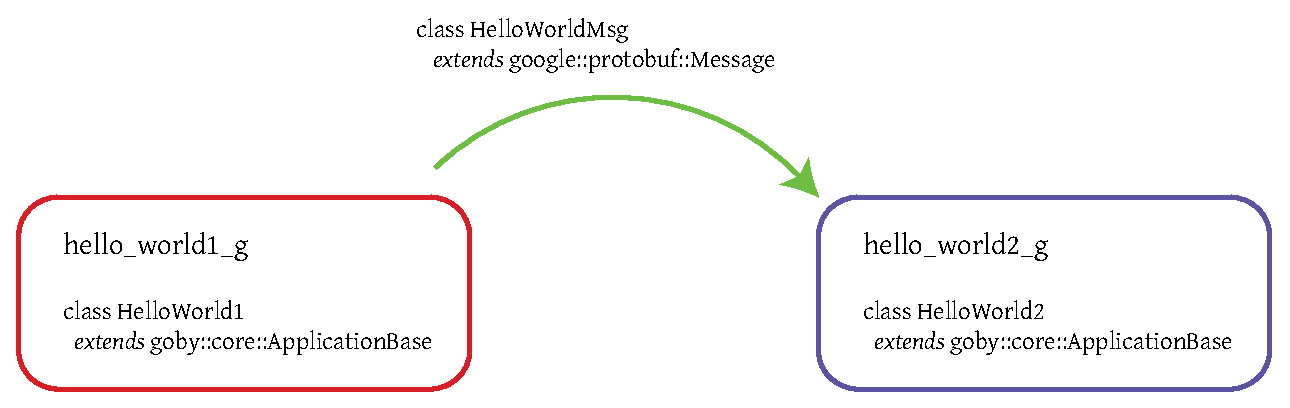
\includegraphics[width=\textwidth]{hello_world_sketch}
\caption{In this example \texttt{hello\_world1\_g} publishes messages of type \texttt{HelloWorldMsg} to the subscriber \texttt{hello\_world2\_g}.}
\label{fig:hello_world_sketch}
\end{figure}

\section{Meeting goby::core::ApplicationBase}

!goby::core::ApplicationBase! is the building block (\gls{base class}) upon which we will make our Goby applications (which will be \glspl{derived class} of ApplicationBase). !ApplicationBase! provides us with a number of tools; the main ones are:

\begin{itemize}
\item a constructor !ApplicationBase()! that reads the command line parameters and the configuration (we will learn about this in Chapter \ref{chap:gps_driver}) and connects to the multicast group for us.
\item a virtual method !loop()! that is called at a regular frequency (10 Hertz by default).
\item a method !subscribe()! which tells !gobyd! that we wish to receive all messages of this type.
\item a method !newest()! which returns the newest (latest received) message of a given type that we have previously called !subscribe()! for. We will learn how to filter the subscriptions later.
\item a method !publish()! allowing us to publish messages to the multicast group and thereby to any subscribers of that type.
\item an object !goby::glog! which acts just like std::cout and lets us write to our choice of debug logs (terminal window / text file) with fine grained control over the verbosity of the output.
\end{itemize}

\section{Creating a simple Google Protocol Buffers Message: HelloWorldMsg}\label{sec:proto_ex}

\glsreset{protobuf} \gls{protobuf} allows us to create custom objects for holding and transmitting data in a structured fashion. Transmitting data typically is done in a long string of bytes. However, humans do not view the world as a string of bytes. We think and communicate using tangible and intangible objects. For example, a baseball might be described by its diameter, color, weight, and materials. Similarly, a sample from a CTD\footnote{Conductivity-Temperature-Depth} sensor can be thought of as an object containing a number of floating point values representing salinity, temperature, pressure, etc. Goby (using protobuf objects) allows messages to be formed using this more natural object-based representation.

The \gls{protobuf} language is simple with a syntax similar to that of C. Protobuf messages are written in .proto files and passed to the protobuf compiler (!protoc!) which generates C++ code to pass to the C++ compiler (!c++!, !gcc! on Linux). See Fig. \ref{fig:hello_world_compile} for a graphical representation of this compilation process. 

\begin{figure}
\centering
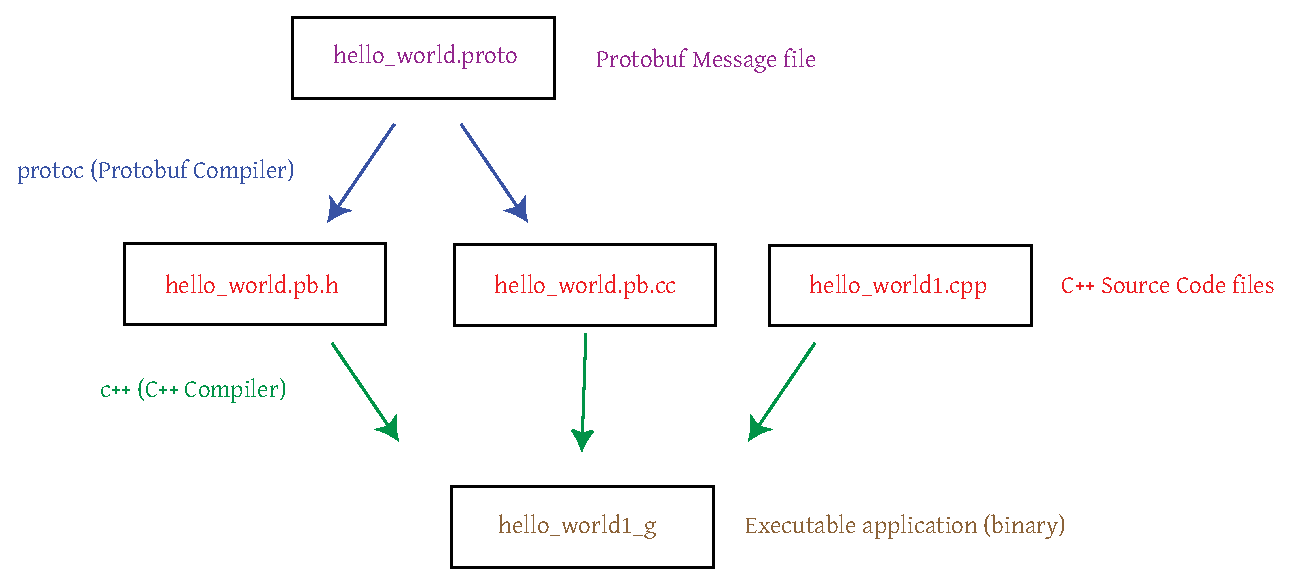
\includegraphics[width=\textwidth]{hello_world_compile}
\caption{The steps of compiling \texttt{hello\_world1\_g.}}
\label{fig:hello_world_compile}
\end{figure}

Protobuf messages can contain a number of basic types (or vectors of these types) as well as nested messages. Fields are labeled as required, optional or repeated (essentially a vector). Required fields must be filled in; clearly, optional fields can be omitted. This might be a good time to read the excellent Protocol Buffers tutorial \cite{proto-tutorial} to get a feel for the language and usage.

As you become familiar with using \gls{protobuf}, the language reference \cite{proto-lang-ref} will help you in creating .proto files and the generated code reference \cite{proto-gen-code} will assist you in accessing the C++ classes created by the !.proto! files when passed through !protoc!.

For this example, we wish to send ``hello world'' (of course) so we need a string to hold our message that we will call `telegram': 
\begin{verbatim}
required string telegram = 1;
\end{verbatim}
The ! = 1! simply indicates that `telegram' is the first field in the message !HelloWorldMsg!. Furthermore, we want to keep track of how many times we've said ``hello'' so we'll add an unsigned integer called `count'
\begin{verbatim}required uint32 count = 2;\end{verbatim}
The resulting .proto file is given in section \ref{sec:hello_world.proto}.

We chose `required' to prefix both fields because we feel that a valid !HelloWorldMsg! must contain both a `telegram' and a `count.' !uint32! is an unsigned (non-negative) 32 bit integer. The numbers following the ``='' sign are unique identifiers for each field. These numbers can be chosen however one likes as long as they are unique within a given protobuf message. Ascending numbers in the order fields are declared in the file is a reasonable choice.

This .proto file is ``compiled'' into a class with the same name as the message (!HelloWorldMsg!). This class is accessed by including a header file with the same name as the .proto file, but with ``.proto'' replaced with ``.pb.h''. Furthermore, we can set the contents of this class using calls (``mutators'' or ``setters'') that are the same as the field name (i.e. `telegram' or `count') prepended with ``set\_'':
\begin{boxedverbatim}
// C++ 
#include "hello_world.pb.h"

// create and populate a ``HelloWorldMsg'' called `msg'
HelloWorldMsg msg;
msg.set_telegram("hello world");
msg.set_count(3);
\end{boxedverbatim}
\resetbvlinenumber

and access them using these methods (``accessors'' or ``getters'') that have the same function name as the field name:

\begin{boxedverbatim}
// C++ 
// print information about `msg' to the screen
std::cout << msg.telegram() << ": " << msg.count() << std::endl;
\end{boxedverbatim}
\resetbvlinenumber


\section{Learning how to \textit{publish}: HelloWorld1}

To create a Goby application, one needs to

\begin{itemize}
\item create a derived class of !goby::core::ApplicationBase!. We also must include the goby core header (!#include "goby/core.h"!).
\item create an overloaded !loop()! method (which can do nothing).
\item run the application using the !goby::run()! function. Because goby::core::ApplicationBase reads our configuration (including command line options) for us, we also pass !argv! and !argc! to !run()!.
\end{itemize}

That is all one needs to create a valid working Goby application. All together the ``bare-bones'' Goby application looks like:

\begin{boxedverbatim}
#include "goby/core.h"

class DoNothingApplication : public goby::core::ApplicationBase 
{
  void loop() {}
};

int main(int argc, char* argv[])
{   
    return goby::run<DoNothingApplication>(argc, argv);
}
\end{boxedverbatim}
\resetbvlinenumber

However, we would like our application to do a little bit more.

ApplicationBase provides a pure \gls{virtual} method called !loop()! that is called on some regular interval (it is the \textit{\gls{synchronous} event} in Goby), by default 10 Hertz. By overloading !loop()! in our derived class !HelloWorld1!, we can do any kind of synchronous work that needs to be done without tying up the CPU all the time\footnote{in between calls to \texttt{loop()}, ApplicationBase handles incoming subscribed messages}. In this example, we will create a simple message (of type !HelloWorldMsg! which we previously designed in section \ref{sec:proto_ex}) and publish it to all subscribers (we create a subscriber in section \ref{sec:sub_ex}). 

Let's walk through each line of our !loop()! method:

\begin{boxedverbatim}
void loop()
{
   static int i = 0;
   HelloWorldMsg msg;
   msg.set_telegram("hello world!");
   msg.set_count(++i);
   goby::glog << "sending: " << msg << std::endl;
   publish(msg);
}
\end{boxedverbatim}
\resetbvlinenumber

\begin{itemize}
\item Line !1!: !loop()! takes no arguments and returns nothing (void). 
\item Line !3!: We declare a static integer\footnote{static in this context means that the variable will keep its value across calls to the function \texttt{loop()}.} to keep track of how many times we have looped and thus print an increasing integer value. 
\item Line !4!: We create an instantiation of !HelloWorldMsg! called !msg!.
\item Line !5!: We set the `telegram` field of the !HelloWorldMsg! named !msg!
\item Line !6!: We set the `count` field of !msg!.
\item Line !7!: We publish a human debugging log message using !goby::glog! (just like std::cout or other std::ostreams), which will be put to the terminal window in verbose mode\footnote{goby provides operator<< for google::protobuf::Message objects as a wrapper for google::protobuf::Message::DebugString()}. 
\item Line !8!: Finally, we publish our message. The entirety of the code for !hello_world1_g! is listed in section \ref{sec:hello_world1.cpp}.

\section{Learning how to \textit{subscribe}: HelloWorld2} \label{sec:sub_ex}

Now that our !hello_world1_g! application is publishing a message, we would like to create an application that subscribes for it. To subscribe for a message, we typically provide two things:
\begin{itemize}
\item The type of the message we want to subscribe for (e.g. !HelloWorldMsg!).
\item A method or function that should be called when we receive a message of that type (a callback).
\end{itemize}

Subscriptions typically take place in the constructor (here, !HelloWorld2::HelloWorld2()!), but can happen at any time as needed (within !loop()!, for example). You subscribe for a type once, and then you will continue to receive all other applications' publishes to that type.

We subscribe for a type using a call to !subscribe()! that looks like this:
\begin{boxedverbatim}
subscribe<HelloWorldMsg>(&HelloWorld2::receive_msg, this);
\end{boxedverbatim}
\resetbvlinenumber

While a bit complicated at first, this call should make sense shortly. It reads ``!subscribe! for all messages of type !HelloWorldMsg! and when you receive one, call the method !HelloWorld2::receive_msg! which is a member of !this! class (!HelloWorld2!).''\footnote{You can call a member function (method) of another class by passing the pointer to the desired class instantiation instead of \texttt{this}. Alternatively, you can call a non-class function by just giving its pointer, e.g. \texttt{subscribe(\&receive\_msg)}.}. The method provided as a callback (here !receive_msg()!) must have the signature
\begin{boxedverbatim}
void func(const ProtoBufMessage&); 
\end{boxedverbatim}
\resetbvlinenumber
where !ProtoBufMessage! is the type subscribed for (here, !HelloWorldMsg!). !receive_msg()! has that signature
\begin{boxedverbatim}
void HelloWorld2::receive_msg(const HelloWorldMsg& msg);
\end{boxedverbatim}
\resetbvlinenumber
and thus is a valid callback for this subscription. After subscribing, !receive_msg()! will be called immediately (an \gls{asynchronous} event) upon receipt of a message of type !HelloWorldMsg! unless
\begin{itemize}
\item !loop()! is in the process of being called or
\item another message callback is in the process of being called.
\end{itemize}
In these cases, !receive_msg()! is called as soon as the blocking method returns. For this example, inside of !receive_msg()! we simply post the message to the debug log:

\begin{boxedverbatim}
void receive_msg(const HelloWorldMsg& msg)
{
   goby::glog << "received: " << msg << std::endl;
}
\end{boxedverbatim}
\resetbvlinenumber

The full source listing for !hello_world2_g! can be found in section \ref{sec:hello_world2.cpp}.

\section{Compiling our applications using CMake}

CMake \cite{cmake}, while still lacking in documentation, is probably the easiest way to build software these days, especially for cross platform support. I will briefly walk through building a Goby application using CMake within the larger Goby project configuration. If you look at the !CMakeLists.txt! file in \ref{sec:hello_world:CMakeLists.txt}, you can see the steps needed to add our new applications to the project:

\begin{boxedverbatim}
protobuf_generate_cpp(PROTO_SRCS PROTO_HDRS hello_world.proto)
add_executable(hello_world1_g hello_world1.cpp ${PROTO_SRCS} ${PROTO_HDRS})
target_link_libraries(hello_world1_g goby_core)
\end{boxedverbatim}
\resetbvlinenumber

Line 1 tells CMake to add ``hello\_world.proto'' to the files needed to be pre-compiled by the Google Protocol Buffers compiler !protoc!. protobuf\_generate\_cpp is provided by the CMake module \href{http://bazaar.launchpad.net/~goby-dev/goby/trunk/annotate/head:/cmake_modules/FindProtobufGoby.cmake}{goby/cmake\_modules/FindProtobufGoby.cmake}. Line 2 adds our application !hello_world1_g! to the list to be compiled by the C++ compiler, using the sources !hello_world1.cpp! and the generated Protocol Buffers code. We append ``\_g'' as a convention to quickly recognize Goby applications. Line 3 links our application against the goby\_core library, which provides goby::core::ApplicationBase, our base class.

Adding !hello_world2_g! is directly analogous.

\section{Trying it all out: running from the command line}

Now, assuming you've compiled everything, we can run the example.

You'll need two terminal windows, one for each of our ``hello world'' applications. Now we can launch our two applications (order doesn't matter), with the added ``-v'' flag to indicate we want verbose terminal output:

\begin{boxedverbatim}
> hello_world1_g -v
> hello_world2_g -v
\end{boxedverbatim}
\resetbvlinenumber

You should see !hello_world1_g! passing messages to !hello_world2_g! every 1/10th second.

\section{Code} \label{sec:hello_example_code}

This entire example can be browsed online at \url{http://bazaar.launchpad.net/~goby-dev/goby/1.0/files/head:/share/examples/core/ex1_hello_world}.

\subsection{goby/share/examples/core/ex1\_hello\_world/hello\_world.proto} \label{sec:hello_world.proto}
\boxedverbatiminput{"../../examples/core/ex1_hello_world/hello_world.proto"}
\resetbvlinenumber

\subsection{goby/share/examples/core/ex1\_hello\_world/hello\_world1.cpp}\label{sec:hello_world1.cpp}
\boxedverbatiminput{"../../examples/core/ex1_hello_world/hello_world1.cpp"}
\resetbvlinenumber

\subsection{goby/share/examples/core/ex1\_hello\_world/hello\_world2.cpp}\label{sec:hello_world2.cpp}
\boxedverbatiminput{"../../examples/core/ex1_hello_world/hello_world2.cpp"}
\resetbvlinenumber
\subsection{goby/share/examples/core/ex1\_hello\_world/CMakeLists.txt}\label{sec:hello_world:CMakeLists.txt}
\boxedverbatiminput{"../../examples/core/ex1_hello_world/CMakeLists.txt"}
\resetbvlinenumber

\DeleteShortVerb{\!}

\chapter{The GPS Driver example} \label{chap:gps_driver}
\MakeShortVerb{\!} % makes !foo! == !foo!
\epigraph{\textit{Man is the best computer we can put aboard a spacecraft, and the only one that can be mass produced with unskilled labor.}}{Werner von Braun}

Robots, like people, need to know where they are. The simplest way now is to use a GPS receiver. While this works only when the robot is on the surface of the ocean, it is one of the most accurate forms of positioning available and thus used as a starting point for undersea dead reckoning using Doppler Velocity Loggers (DVLs) or Inertial Measurement Units (IMUs). Therefore, reading a GPS receiver's output into a usable form for decision making is a useful and necessary ability for our marine robot. This example shows how we might do this using Goby by making an application !gps_driver_g!.

Typically we might also need to know the depth of our vehicle. This is often determined by measuring the ambient pressure. In this example, we will simulate the scalar depth reading of such a pressure sensor in !depth_simulator_g!.

Finally, it is often useful to have an aggregate of the vehicle's status that includes a snapshot of the vehicle's location, orientation, speed, heading, and perhaps other factors such as battery life and health. For this example, we call such a message a !NodeReport! and provide an application !node_reporter_g! that compiles the reports from the GPS and the depth sensor into a single message. To extend this example, we could add data from other sources, such as an inertial measurement unit (IMU) or Doppler Velocity Logger (DVL).

As the first example, the files for this example are located at the end of the chapter in section \ref{sec:gps_driver_example_code}.

\section{Reading \textit{configuration} from files and command line: DepthSimulator}

!DepthSimulator! reads a starting depth value from a configuration file and reports that value as the current depth, perturbed slightly by a random value. It's a primitive constant depth simulator, but allows us to illustrate another feature of Goby, the configuration file reader.

Goby reads configuration text files and the command line using \gls{protobuf}, in a similar manner messages are defined for passing between applications. The Goby application author provides a !.proto! file containing a protobuf message that defines all possible valid configuration values for the given application in the form of a protobuf message. Then the application instantiates a copy of this configuration message and passes it to the !goby::core::ApplicationBase! constructor with reads the configuration text file and/or command line options. If the configuration text file and/or command line options properly populate the provided proper configuration protobuf message, the message is returned to the derived class (the Goby application). Otherwise, execution of the application ends with a useful error message for the user explaining the errors involved with the passed configuration. 

Thus, for the !DepthSimulator! we define a protobuf message called !DepthSimulatorConfig!:
\begin{boxedverbatim}
message DepthSimulatorConfig
{
  required AppBaseConfig base = 1;
  required double depth = 2;
}
\end{boxedverbatim}
\resetbvlinenumber

An embedded message of type !AppBaseConfig! is always provided for configuring parameters common for all Goby applications, such as the frequency that the virtual method !loop()! is called, the name (alias) that the application is to use to communicate (if different from the compiled name), and the connection details (IP addresses, ports, etc.). The !AppBaseConfig! message is defined in goby/src/core/proto/app\_base\_config.proto.

Specifically, for our !DepthSimulator!, we only have one other configuration parameter, a double called `depth'. It is required, so our application will fail to run without a depth provided.

To use the Goby configuration reader, we create an instantation of our !DepthSimulatorConfig!
\begin{boxedverbatim}
class DepthSimulator : public goby::core::ApplicationBase
{ 
...
    static DepthSimulatorConfig cfg_;
};
\end{boxedverbatim}
\resetbvlinenumber
which must either be a global object or a static member of our class\footnote{The configuration object must be a static member so that it is instantiated \textit{before} the \texttt{goby::core::ApplicationBase} since normal members of our \texttt{DepthSimulator} class would be instantiated \textit{after} \texttt{ApplicationBase}, which would lead to trouble when \texttt{ApplicationBase} tried to use the object.}.

Then, all we must do is pass a pointer to that object to the constructor of the base class:
\begin{boxedverbatim}
    DepthSimulator()
        : goby::core::ApplicationBase(&cfg_)
\end{boxedverbatim}
\resetbvlinenumber
!goby::core::ApplicationBase! will take of the rest. To see what configuration values (with the correct syntax) can be used in our compiled !depth_simulator_g!, we can run it with the !-e! flag:

\begin{boxedverbatim}
> depth_simulator_g -e
\end{boxedverbatim}
\resetbvlinenumber

which gives us a good list of options to choose from. For many of these, the defaults will be fine for now.
\begin{boxedverbatim}
base {  #  (req)
  ethernet_address: "127.0.0.1"  # primary IP address of the 
                                 # interface to multicast over 
                                 # (opt) (default="127.0.0.1")
  multicast_address: "239.255.7.15"  # multicast IP address to 
                                     # use; 
                                     # 239.252.0.0-239.255.255.255 
                                     # is recommended (site-local). 
                                     # See also 
                                     # http://www.iana.org/assignmen
                                     # ts/multicast-addresses/multic
                                     # ast-addresses.xml (opt) 
                                     # (default="239.255.7.15")
  ethernet_port: 11142  #  (opt) (default=11142)
  platform_name: "unnamed_goby_platform"  # same as self.name for 
                                          # gobyd cfg (opt) 
                                          # (default="unnamed_goby_p
                                          # latform")
  app_name: "myapp_g"  # default is compiled name - change this 
                       # to run multiple instances (opt)
  verbosity: QUIET  # Terminal verbosity (QUIET, WARN, VERBOSE, 
                    # GUI, DEBUG1, DEBUG2, DEBUG3) (opt) 
                    # (default=QUIET)
  using_database: true  # True if using goby_database, false if 
                        # no database is to be run (opt) 
                        # (default=true)
  database_address: "127.0.0.1"  # TCP address to send database 
                                 # requests on. If omitted and 
                                 # using_database==true, 
                                 # `ethernet_address` is used (opt)
  database_port: 11142  # TCP port to send database requests on. 
                        # If omitted and using_database==true, 
                        # `ethernet_port` is used (opt)
  loop_freq: 10  # the frequency (Hz) used to run loop() (opt) 
                 # (default=10)
}
depth:   #  (req)
\end{boxedverbatim}
\resetbvlinenumber



Similarly, to see the allowed command line parameters we can run it with the !-h! (or equivalently, !--help!) flag:
\begin{boxedverbatim}
> depth_simulator_g --help
\end{boxedverbatim}
\resetbvlinenumber

which should provides output\footnote{Some of the options are removed for brevity}:
\begin{boxedverbatim}
Allowed options:

Typically given in depth_simulator_g configuration file,
but may be specified on the command line:
  --depth arg            (req)

Given on command line only:
  -c [ --cfg_path ] arg    path to depth_simulator_g configuration file 
                           (typically depth_simulator_g.cfg)
  -h [ --help ]            writes this help message
  -a [ --app_name ] arg    name to use while communicating in goby (default: 
                           ./depth_simulator_g)
  -e [ --example_config ]  writes an example .pb.cfg file
  -v [ --verbose ] arg     output useful information to std::cout. -v is 
                           verbosity: verbose, -vv is verbosity: debug1, -vvv 
                           is verbosity: debug2, -vvvv is verbosity: debug3
  -n [ --ncurses ]         output useful information to an NCurses GUI instead 
                           of stdout. If set, this parameter overrides 
                           --verbose settings.
  -d [ --no_db ]           disables the check for goby_database before 
                           publishing. You must set this if not running the 
                           goby_database.
\end{boxedverbatim}
\resetbvlinenumber

Thus, to configure !depth_simulator_g! I could create a text file (let's say depth\_simulator.cfg) with values like
\begin{boxedverbatim}
# depth_simulator.cfg
base
{
    platform_name: "AUV-1"
    loop_freq: 1
}

depth: 10.4
\end{boxedverbatim}
\resetbvlinenumber

Then, when we run !depth_simulator_g! we pass the path to the configuration file as the first command line option:
\begin{boxedverbatim}
> depth_simulator_g depth_simulator.cfg 
\end{boxedverbatim}
\resetbvlinenumber

If we didn't want to use a configuration file, we could pass the same contents of the depth\_simulator.cfg file given above on the command line instead:
\begin{boxedverbatim}
> depth_simulator_g --base 'platform_name: "AUV-1" loop_freq: 1' --depth 10.4
\end{boxedverbatim}
\resetbvlinenumber

If the same configuration values are provided in both the configuration file and on the command line, they are merged for ``repeat'' fields. For ``required'' or ``optional'' fields, the command line value overwrites the configuration file value. 

Thus, if we run
\begin{boxedverbatim}
> depth_simulator_g depth_simulator.cfg --depth 20.5
\end{boxedverbatim}
\resetbvlinenumber
!cfg_.depth()! is 20.5 since the command line provided value takes precedence.

Some commonly used configuration values have shortcuts for the command line. For example, the following two commands are equivalent ways to set the platform name:
\begin{boxedverbatim}
> depth_simulator_g --base 'platform_name: "AUV-1"'
> depth_simulator_g -p "AUV-1"
\end{boxedverbatim}
\resetbvlinenumber

Other than reading a configuration file, all !DepthSimulator! does is repeatedly write a message of type !DepthReading! (see section \ref{sec:gps_driver:depth_reading.proto}) based off a random offset to the configuration value ``depth'':
\begin{boxedverbatim}
void loop()
    {
       DepthReading reading;
       // just post the depth given in the configuration file plus a small random offset
       reading.set_depth(cfg_.depth() + (rand() % 10) / 10.0);

       glogger() << reading << std::flush;
       publish(reading);    
    }
\end{boxedverbatim}
\resetbvlinenumber

You will note that depth\_reading.proto contains an import command and a field of type `Header':
\begin{boxedverbatim}
import "goby/core/proto/header.proto";

message DepthReading
{
  // time is in header
  required Header header = 1;
  required double depth = 2;
}
\end{boxedverbatim}
\resetbvlinenumber

`Header' (defined in goby/src/core/proto/header.proto) provides commonly used fields such as time and source / destination addressing. It is highly recommended to include this in messages sent through Goby, but not required. !goby::core::ApplicationBase! will populate any required fields in `Header' not given by DepthSimulator. For example, if the `time' is not set, !goby::core::ApplicationBase! will set the time based on the time !publish()! was called. However `time' should be set if the calling application has a better time stamp for the message than the publish time (for example, the time a sensor's sample was taken).

\section{Our first \textit{useful} application: \texttt{GPSDriver}}

!GPSDriver! doesn't introduce any new features of Goby, but it attempts to be the first non-trivial application we have seen thus far. !GPSDriver! connects to a NMEA-0183 compatible GPS receiver over a serial port, reads all the messages and parses the GGA sentence into a useful protobuf message for posting to the database.

\subsection{Configuration}
The configuration needed for !GPSDriver! all pertains to how the serial GPS receiver is connected and how it communicates:
\begin{boxedverbatim}
message GPSDriverConfig
{
  required AppBaseConfig base = 1;

  required string serial_port = 2;
  optional uint32 serial_baud = 3 [default = 4800];
  optional string end_line = 4 [default = "\r\n"];
}
\end{boxedverbatim}
\resetbvlinenumber

Note the use of defaults when they are meaningful (the NMEA-0183 specification requires carriage return (!\r!) and new line (!\n!) to signify the end of a line so this default will likely often be precisely what our users want, saving them the effort of specifying it every time).

\subsection{Protobuf Messages}
GPSDriver uses two \gls{protobuf} messages both defined in gps\_nmea.proto (see section \ref{sec:gps_driver:gps_nmea.proto}). The first (!NMEASentence!) is a parsed version of a generic NMEA-0183 message. The second (!GPSSentenceGGA!) contains a !NMEASentence! but also the parsed fields of the GGA position message. Providing the !GPSSentenceGGA! gives all subscribers of this message rapid access to useful data without parsing the original NMEA string again.

\subsection{Body}
!GPSDriver! should be straightforward to understand given what we have learned to this point. It makes use of some utilities in the goby::util libraries, especially the !goby::util::SerialClient! used for reading the serial port. These utilities are documented along with all the other Goby classes at \url{http://gobysoft.com/doc}.

Goby makes heavy use of the Boost libraries (\url{http://www.boost.org}). While you are not required to use any of Boost when developing Goby applications, it would be worth your while becoming acquainted with them. For example, the Boost Date-Time library gives a handy object oriented way to handle dates and times that far exceeds the abilities of ctime (i.e. time.h).

\section{Subscribing for \textit{multiple types}: NodeReporter}

!NodeReporter! subscribes to both the output of !DepthSimulator! (!DepthReading!) and !GPSDriver! (!GPSSentenceGGA!). Whenever either is published, a new !NodeReport! message is created as the aggregate of pieces of both messages. The !NodeReport! (defined in node\_report.proto in section \ref{sec:gps_driver:node_report.proto}) is a useful summation of the status of a given node (synonomously, platform). Because !DepthReading! and !GPSSentenceGGA! are published asynchronously, we also keep track of the delays between different parts of the NodeReport message (the !*_lag! fields). 

The !NodeReport! provides
\begin{enumerate}
\item Name of the platform
\item Type of the platform (e.g. AUV, buoy)
\item The global position of the vehicle in geodetic coordinates (latitude, longitude, depth)
\item The local position of the vehicle in a local cartesian coordinate system (x, y, z) based off the datum defined in the configuration. This is generally more useful for vehicle operators than the global fix.
\item The Euler angles of the current vehicle pose: roll, pitch, yaw (heading). 
\item The speed of the vehicle.
\end{enumerate}

In this example, we only set the first three fields given above. The others would require further sensing capability than we have in this example.

\section{Putting it all together}

First, we either need a real GPS unit or simulate one somehow. If you have a real NMEA-0183 GPS handy, by all means use it. Otherwise, I've made a fake GPS using !socat! and a log file of a real GPS (nmea.txt). This fake GPS can be run using
\begin{verbatim}
./fake_gps.sh nmea.txt
\end{verbatim}
which writes a line from nmea.txt every second to the fake serial port !/tmp/ttyFAKE!. This should be good enough for us here. If you don't have !socat!, you should be able to find it in the package manager for your Linux distribution (!sudo apt-get install socat! in Debian or Ubuntu).

Next we need to launch everything. The list is beginning to grow
\boxedverbatiminput{"../../examples/core/ex2_gps_driver/launch_list.txt"}
\resetbvlinenumber
but fortunately we've provided a script that launches everything for you in separate terminal windows. So all you need to do is type
\begin{boxedverbatim}
./launch.sh
\end{boxedverbatim}
\resetbvlinenumber
and enjoy the magic unfold. Should you wish to modify how things are launched, just edit launch\_list.txt in goby/share/examples/core/ex2\_gps\_driver.

\section{Reading the log files (SQLite3)}

You may have noticed that everytime you run !gobyd! it creates a log file called !AUV-1_YYYYMMDDTHHMMSS_goby.db!. This is an SQLite3 \cite{sqlite} \gls{sql} database. Every variable published in Goby is written to this database. To read it, you need a tool capable of reading SQLite3 databases. One candidate is the !sqlite3! command line tool. The following will dump to your screen all the DepthReading values recorded. Using the interactive mode:
\begin{boxedverbatim}
sqlite3 AUV-1_20110304T212549_goby.db
sqlite> .mode column
sqlite> .headers ON
sqlite> SELECT * FROM DepthReading;
\end{boxedverbatim}
\resetbvlinenumber
or similarly on the command line only
\begin{boxedverbatim}
sqlite3 -header -column AUV-1_20110304T212549_goby.db "SELECT * FROM DepthReading"
\end{boxedverbatim}
\resetbvlinenumber

If a Graphical User Interface (GUI) is more your style, \url{http://www.sqlite.org/cvstrac/wiki?p=ManagementTools} has a whole list. My preference is Sqliteman, accessible in Ubuntu with !sudo apt-get install sqliteman!. Then it's just a matter of loading up the database and away you go:
\begin{boxedverbatim}
sqliteman AUV-1_20110304T212549_goby.db
\end{boxedverbatim}
\resetbvlinenumber

\section{Code} \label{sec:gps_driver_example_code}

This entire example can be browsed online at \url{http://bazaar.launchpad.net/~goby-dev/goby/1.0/files/head:/share/examples/core/ex2_gps_driver}.

\subsection{goby/share/examples/core/ex2\_gps\_driver/config.proto} \label{sec:gps_driver:config.proto}
\boxedverbatiminput{"../../examples/core/ex2_gps_driver/config.proto"}
\resetbvlinenumber

\subsection{goby/share/examples/core/ex2\_gps\_driver/depth\_reading.proto} \label{sec:gps_driver:depth_reading.proto}
\boxedverbatiminput{"../../examples/core/ex2_gps_driver/depth_reading.proto"}
\resetbvlinenumber

\subsection{goby/share/examples/core/ex2\_gps\_driver/depth\_simulator.cpp} \label{sec:gps_driver:depth_simulator.cpp}
\boxedverbatiminput{"../../examples/core/ex2_gps_driver/depth_simulator.cpp"}
\resetbvlinenumber

\subsection{goby/share/examples/core/ex2\_gps\_driver/node\_report.proto} \label{sec:gps_driver:node_report.proto}
\boxedverbatiminput{"../../examples/core/ex2_gps_driver/node_report.proto"}
\resetbvlinenumber


\subsection{goby/share/examples/core/ex2\_gps\_driver/node\_reporter.h} \label{sec:gps_driver:node_reporter.h}
\boxedverbatiminput{"../../examples/core/ex2_gps_driver/node_reporter.h"}
\resetbvlinenumber


\subsection{goby/share/examples/core/ex2\_gps\_driver/node\_reporter.cpp} \label{sec:gps_driver:node_reporter.cpp}
\boxedverbatiminput{"../../examples/core/ex2_gps_driver/node_reporter.cpp"}
\resetbvlinenumber


\subsection{goby/share/examples/core/ex2\_gps\_driver/gps\_nmea.proto} \label{sec:gps_driver:gps_nmea.proto}
\boxedverbatiminput{"../../examples/core/ex2_gps_driver/gps_nmea.proto"}
\resetbvlinenumber

\subsection{goby/share/examples/core/ex2\_gps\_driver/gps\_driver.h} \label{sec:gps_driver:gps_driver.h}
\boxedverbatiminput{"../../examples/core/ex2_gps_driver/gps_driver.h"}
\resetbvlinenumber
\subsection{goby/share/examples/core/ex2\_gps\_driver/gps\_driver.cpp} \label{sec:gps_driver:gps_driver.cpp}
\boxedverbatiminput{"../../examples/core/ex2_gps_driver/gps_driver.cpp"}
\resetbvlinenumber

\subsection{goby/share/examples/core/ex2\_gps\_driver/gobyd.cfg} \label{sec:gps_driver:gobyd.cfg}
\boxedverbatiminput{"../../examples/core/ex2_gps_driver/gobyd.cfg"}
\resetbvlinenumber

\subsection{goby/share/examples/core/ex2\_gps\_driver/depth\_simulator\_g.cfg} \label{sec:gps_driver:depth_simulator_g.cfg}
\boxedverbatiminput{"../../examples/core/ex2_gps_driver/depth_simulator_g.cfg"}
\resetbvlinenumber

\subsection{goby/share/examples/core/ex2\_gps\_driver/gps\_driver\_g.cfg} \label{sec:gps_driver:gps_driver_g.cfg}
\boxedverbatiminput{"../../examples/core/ex2_gps_driver/gps_driver_g.cfg"}
\resetbvlinenumber

\subsection{goby/share/examples/core/ex2\_gps\_driver/node\_reporter\_g.cfg} \label{sec:gps_driver:node_reporter_g.cfg}
\boxedverbatiminput{"../../examples/core/ex2_gps_driver/node_reporter_g.cfg"}
\resetbvlinenumber

\subsection{goby/share/examples/core/ex2\_gps\_driver/nmea.txt} \label{sec:gps_driver:nmea.txt}
\boxedverbatiminput{"../../examples/core/ex2_gps_driver/nmea.txt"}
\resetbvlinenumber

\DeleteShortVerb{\!}

\chapter{What's next}

That's all for \verb|goby| in Release 2.0. There's still a lot to do so keep tuned. If you want the bleeding edge, you can check out the Goby 3.0 branch with 
\verb|bzr checkout lp:goby/3.0|.

Here's what's on the horizon:
\begin{itemize}
\item Goby-Common: a general purpose interprocess and interplatform communication based on messaging schemes drawn both from the existing marine robotics and global open source communities. The focus is on a high degree of runtime reliability and collaboration between development communities. For advanced users, it provides a transport layer built on ZeroMQ (which supports 20+ languages including C, C++, Java, .NET, Python, and major platforms) for communicating over reliable multicast (PGM) using one or more existing (e.g. MOOS, LCM, Protobuf, CCL, DCCL, ...) messaging schemes. Goby does not mandate a programming language, a messaging scheme, or a development system and thus intends to tie together groups with different goals, styles, and rules. Furthermore, Gateways can be written to interface the ZeroMQ based Goby transport with the native transport systems used by other architectures (e.g. MOOSDB, LCM multicast).
\item Goby-PB: The Google Protocol Buffers / C++ implementation of Goby-Common. For introductory users, it provides an "template" application in C++ that allows object-based messaging (based on Google Protocol Buffers) between processes and platforms without any concern for serialization, routing, sockets, and so on.
\end{itemize}

Stay tuned at \url{https://launchpad.net/goby}. Thanks.


\appendix

\chapter{Goby MOOS Modules}\label{chap:MOOS}
\MakeShortVerb{\!} % makes !foo! == !foo!

The acoustic communications portion of Goby was developed originally for the MOOS autonomy architecture. Thus, the relevant MOOS modules !pAcommsHandler! and others are still maintained (in goby/src/moos) for the use of the !MOOS-IvP! community. !MOOS-IvP! is explained in \cite{moos-ivp-jfr} and is available at \url{http://moos-ivp.org}. The usage of these modules is documented here. See \url{http://gobysoft.org/wiki/InstallingGoby} for how to install Goby.


\section{Goby MOOS Applications} \label{sec:goby_moos_app}

The Goby MOOS applications share a common subclass of CMOOSApp that provides a validating configuration reader based on the Google Protocol Buffers TextFormat class. The configuration is still embedded within the .moos file, but the syntax is somewhat different. Here you can control logging to a text file and terminal verbosity. You can also initialize a variable in the MOOS database at startup. Many of these parameters will automatically be set to a global MOOS variable (specified outside any ProcessConfig block) if left empty. For example, the global MOOS variable !LatOrigin! will set the Goby MOOS configuration variable !common::lat_origin!. This allows Goby MOOS applications to conform to MOOS \textit{de facto} conventions.

Any Goby MOOS application will give all its valid configuration parameters with \begin{verbatim}
> pGobyApp --example_config
\end{verbatim} 

\boxedverbatiminput{@RELATIVE_CMAKE_CURRENT_SOURCE_DIR@/includes/common.pb.cfg}
\resetbvlinenumber

Some details about the configuration values:

\begin{itemize}
\item !log!: boolean to indicate whether to log terminal output or not to files in the path by !log_path!.
\item !log_path!: folder to log all terminal output to for later debugging. Similar to system logs in /var/log.
\item !log_verbosity!: verbosity of the log file. See !verbosity! for the various settings.
\item !community!: the name of the current vehicle community. If omitted, read from the !Community=! global MOOS configuration field.
\item !lat_origin!: a decimal degrees latitude indicating the local cartesian origin. If omitted, read from the !LatOrigin=! global MOOS configuration field.
\item !lon_origin!: a decimal degrees longitude indicating the local cartesian origin. If omitted, read from the !LongOrigin=! global MOOS configuration field.
\item !app_tick!: same as AppTick.
\item !comm_tick!: same as CommsTick.
\item !verbosity!: choose !DEBUG1!-!DEBUG3! for various levels of debugging output, !VERBOSE! for some text terminal output, !WARN! for warnings only, and !QUIET! for no terminal output.
\item !show_gui!: if true, the running terminal opens an NCurses GUI helpful to debugging and visualizing the many data flows of pAcommsHandler. The verbosity in this GUI is governed by !verbosity!.
\item !initializer!: since many times it is useful to have a MOOS variable including in a message that remains static for a given mission (vehicle name, etc), we give the option to publish initial MOOS variables here (for later use in messages [until overwritten, of course]). If !global_cfg_var! is set, pAcommsHandler looks for a global (i.e. specified at the top of the MOOS file or outside any !ProcessConfig! blocks) value in the .moos file with the name to the right of the colon and publishes it to a MOOS variable with the name to the left of the colon. For example:
\begin{verbatim}
initializer { global_cfg_var: "LatOrigin" moos_var: "LAT_ORIGIN" } 
\end{verbatim}
\resetbvlinenumber
looks for a variable in the .moos file called !LatOrigin! and publishes it to the MOOSDB as a double variable !LAT_ORIGIN! with the value given by !LatOrigin!.
\end{itemize}


\section{pAcommsHandler}
\label{sec:pacommshandler} 

pAcommsHandler provides a:
\begin{enumerate}
\item MOOS Application wrapper for the Goby-Acomms communication library.
\item set of translation tools for converting the DCCL messages (written as an extension of Google Protocol Buffers) to MOOS types (strings and doubles) and vice-versa.
\item full backwards-compatibility support module for version 1 XML messages. 
\end{enumerate}

This section describes only the parts relevant for interface to MOOS (variables and translator entries that allow you to read and write to and from DCCL (Protobuf) messages). You should read Chapter \ref{chap:acomms} before starting this section and reference it as necessary.

\subsection{Parameters for the pAcommsHandler Configuration Block}\label{sec:pAcommsHandler:config}

\subsubsection{Example moos file}

pAcommsHandler has a large number of configuration options, many of which you will never use or leave as default. You can always get a complete listing of MOOS file parameters with their syntax by running
\begin{verbatim}
> pAcommsHandler --example_config
\end{verbatim}
\resetbvlinenumber

These configuration values are provided here (with $\ldots$ where the relevant configuration is provided elsewhere in this document):

\boxedverbatiminput{@RELATIVE_CMAKE_CURRENT_SOURCE_DIR@/includes/pAcommsHandler_reduced.moos}
\resetbvlinenumber


\subsubsection{Filling out the .moos file}\label{sec:pAcommsHandler_moos_file}

Many of the parameters are sufficiently explained in the above list of configuration parameters. What follows is a detailed explanation of the parameters that need further explanation.

\begin{itemize}
\item !common!: Parameters that can be set for any of the Goby MOOS applications. See section \ref{sec:goby_moos_app}.
\item !modem_id!: integer that specifies the !modem_id! of this current vehicle / community. For the WHOI Micro-Modem this is the Micro-Modem ``SRC'' configuration parameter (as set by !$CCCFG,SRC,#!). For the remainder of the document, !modem_id! refers to the value !$CCCFG,SRC,modem_id!. This configuration parameter will be set on startup. Setting this within the main block for pAcommsHandler sets it for all the modules (!driver_cfg!, !queue_cfg!, !mac_cfg!) 
\item !driver_type!: 
\begin{itemize}
\item !DRIVER_WHOI_MICROMODEM! is a driver for the WHOI Micro-Modem. 
\item !DRIVER_ABC_EXAMPLE_MODEM! is a simple test ``modem''. Do not use this for real work, but rather for learning how to write new drivers for Goby.
\item !DRIVER_UFIELD_SIM_DRIVER! is a driver for the MOOS-IvP uField toolbox.
\item !DRIVER_PB_STORE_SERVER! is a ZeroMQ (TCP, UNIX sockets) driver for the !goby_store_server! database.
\item !DRIVER_UDP! is a user datagram protocol (UDP) driver. This is probably the easiest driver to start with for learning pAcommsHandler.
\item !DRIVER_NONE! disables the modem driver.
\end{itemize}
\item !driver_cfg!: Configures the base driver and the specific driver selected. See section \ref{sec:driver}.
\item !mac_cfg!: Configures the acoustic Medium Access Control. See section \ref{sec:amac}.
\item !queue_cfg!: Configures the Priority Queuing layer. See section \ref{sec:queue}.
\item !dccl_cfg!: Configures the Dynamic Compact Control Language. See section \ref{sec:dccl}.
\item !route_cfg!: Configures a basic static routing module. This is experimental and subject to change.
\item !moos_var!: Rename any or all of the MOOS variables published by pAcommsHandler.
\item !load_shared_library!: List of paths to shared libraries containing compiled DCCL (Google Protocol Buffers) messages.
\item !load_proto_file!: List of paths to .proto files containing compiled DCCL (Google Protocol Buffers) messages. These will be compiled at runtime and loaded. It is preferable to use !load_shared_library! when possible, as syntactical and type mistakes in the DCCL messages will be caught at compile-time rather than delayed to runtime.
\item !translator_entry!: List of entries indicating when to make (\textit{trigger}) and how to \textit{create} outgoing DCCL messages, and how to \textit{publish} incoming DCCL messages. This can be thought of as providing a generic interface between MOOS strings and Google Protocol Buffers messages.
\item !multiplex_create_moos_var!: Used by !goby_liaison! to publish multiple commands (outgoing messages) on a single MOOS variable.
\item !modem_id_lookup_path!: path to a text file giving the mapping between !modem_id! and vehicle name and type for a given experiment. This file should look like:
\begin{boxedverbatim}
// modem id, vehicle name (should be community name), vehicle type
0, broadcast, broadcast
1, endeavor, ship
3, unicorn, auv
4, macrura, auv
\end{boxedverbatim}
\resetbvlinenumber
\item !transitional_cfg!: Provides the same functionality as !dccl_cfg! does in pAcommsHandler from version 1 of Goby. Behind the scenes, XML messages are read, translated to version 2 Protobuf DCCL messages, and written to the !generated_proto_dir!, and subsequently loaded using !load_proto_file!. The appropriate !translator_entry!s are also created from these messages. Do not use this configuration or the XML representation of DCCL messages for any new projects. See the version 1 documentation (\url{http://gobysoft.org/doc/1.1/}) for more details on the XML representation of DCCL messages.
\end{itemize}

%\subsection{MOOS variables subscribed to by pAcommsHandler}
%
%Except for the user-configured publishes (!translator_entry!), pAcommsHandler uses the \href{http://code.google.com/apis/protocolbuffers/docs/reference/cpp/google.protobuf.text_format.html}{Google Protocol Buffers TextFormat} class for serializing to and parsing from MOOS strings (same as !TECHNIQUE_PREFIXED_PROTOBUF_TEXT_FORMAT!). This saves significant effort in manually parsing strings. You should use these same facilities for creating and reading messages. Two helper functions are provided in \\ \href{http://gobysoft.com/doc/moos__protobuf__helpers_8h.html}{goby/moos/libmoos\_util/moos\_protobuf\_helpers} will help you serialize and parse these messages. See \url{http://gobysoft.com/doc/2.0/acomms.html#protobuf} for a brief overview of Google Protocol Buffers as used in Goby.
%
%\begin{itemize}
%\item !DCCL!: Most variables subscribed to by pAcommsHandler are configured in the message XML files and are designated by the tags \xmltag{src\_var} (used to fetch data for a particular !message_var! within a DCCL message) and \xmltag{trigger\_var} (used to trigger the creatinon of a particular DCCL message and possibly provide some data for that message. See \ref{sec:dccl_overview} for details on the XML configuration. 
%\item !Queue!:
%\begin{itemize}
%\item Subscribes to the variables given in !queue_cfg.queue.in_pubsub_var! for CCL queue sending. The contents of this MOOS variable should be a serialized \href{http://gobysoft.com/doc/modem__message_8proto_source.html}{ModemDataTransmission}). 
%\item !ACOMMS_RANGE_COMMAND! (type: \href{http://gobysoft.com/doc/modem__message_8proto_source.html}{ModemRangingRequest}): You write this to initiate a ranging request outside the MAC schedule. Note in general it is preferable to use the MAC cycle to coordinate data and ranging.
%\end{itemize}
%\item !MAC!: !ACOMMS_MAC_CYCLE_UPDATE! (type: \href{http://gobysoft.com/doc/amac_8proto_source.html}{MACUpdate}) You write this to update the MAC cycle for !MAC_FIXED_DECENTRALIZED! and !MAC_POLLED! modes of operation.
%\end{itemize}
%
%For example, to publish a !ACOMMS_MAC_CYCLE_UPDATE!, you would use code like this:
%\begin{boxedverbatim}
%// provides serialize_for_moos
%#include <goby/moos/libmoos_util/moos_protobuf_helpers.h>
%// provides goby::acomms::protobuf::MACUpdate
%#include <goby/common/amac.pb.h>
%
%...
%
%MyMOOSApp::Iterate()
%{
%  if(do_update_mac)
%  { 
%    using namespace goby::acomms::protobuf;
%    MACUpdate mac_update;
%    mac_update.set_dest(1); // update for us if modem_id == 1
%    // add slot to end of existing cycle
%    mac_update.set_update_type(MACUpdate::ADD);
%    Slot* new_slot = mac_update.add_slot();
%    new_slot->set_src(1);  // send from us
%    new_slot->set_dest(3); // send to vehicle 3
%    new_slot->set_rate(0);
%    new_slot->set_slot_seconds(15);
%    new_slot->set_type(SLOT_DATA);
%    
%    std::string serialized;
%    serialize_for_moos (&serialized, mac_update);
%    m_Comms.Notify("ACOMMS_MAC_CYCLE_UPDATE", serialized);
%  }
%}
%\end{boxedverbatim}
%\resetbvlinenumber
%
%\subsection{MOOS variables published by pAcommsHandler}
%
%Except for DCCL \xmltag{publish\_var}s (which use a printf style syntax), pAcommsHandler uses the Google Protocol Buffers TextFormat class for serializing to MOOS strings. 
%
%\begin{itemize}
%\item !DCCL!: Most variables published by pAcommsHandler are configured in the message XML files and are designated by the tags \xmltag{publish\_var} within a \xmltag{publish} block. See \ref{sec:dccl_overview} for details on the XML configuration. 
%\item !Queue!:
%\begin{itemize}
%\item !ACOMMS_INCOMING_DATA! (type: \href{http://gobysoft.com/doc/modem__message_8proto_source.html}{ModemDataTransmission}) written for all received messages containing a data payload
%\item !ACOMMS_OUTGOING_DATA! (type: \href{http://gobysoft.com/doc/modem__message_8proto_source.html}{ModemDataTransmission}) written for all queued messages containing a data payload
%\item !ACOMMS_RANGE_RESPONSE! (type: \href{http://gobysoft.com/doc/modem__message_8proto_source.html}{ModemRangingReply}) written in response to ranging request (to another modem or LBL beacons)
%\item !ACOMMS_ACK! (type: \href{http://gobysoft.com/doc/modem__message_8proto_source.html}{ModemDataAck}) written when received data is acknowledged acoustically by a third party. Contains the original message.
%\item !ACOMMS_EXPIRE! (type: \href{http://gobysoft.com/doc/modem__message_8proto_source.html}{ModemDataExpire}) written when a message expires (time-to-live [ttl] exceeded) from the queue before being sent (ack = false) or acknowledged (ack = true)
%\item !ACOMMS_QSIZE! (type: \href{http://gobysoft.com/doc/queue_8proto_source.html}{QueueSize}) written when a queue changes size (pop or push) with the new size of the queue.
%\end{itemize}
%\item !MAC!: Does not publish anything.
%\item !ModemDriver!: 
%\begin{itemize}
%\item !ACOMMS_NMEA_IN! (type: string), ModemMsgBase::raw() for all incoming messages ("\$CA..." for WHOI Micro-Modem)
%\item !ACOMMS_NMEA_OUT! (type: string), ModemMsgBase::raw() for all outgoing messages ("\$CC..." for WHOI Micro-Modem)
%\end{itemize}
%\end{itemize}
%
%For example, to read an !ACOMMS_RANGE_RESPONSE!, you would use code like this:
%\begin{boxedverbatim}
%// provides parse_for_moos
%#include <goby/moos/libmoos_util/moos_protobuf_helpers.h>
%// provides goby::acomms::protobuf::ModemRangeReply
%#include <goby/common/modem_message.pb.h>
%
%...
%
%MyMOOSApp::OnNewMail()
%{
%  ...
%  if(moos_msg.GetKey() == "ACOMMS_RANGE_RESPONSE")
%  {
%    using namespace goby::acomms::protobuf;
%    ModemRangeReply range_response;
%    parse_for_moos (serialized, &range_response);
%    
%    // now do what you want to with the nice `range_response` object
%    std::cout << "one way travel time to " << range_response.base().dest() 
%              << " is " << range_response.one_way_travel_time(0) << std::endl;
%  }
%}
%\end{boxedverbatim}
%\resetbvlinenumber
%
%\subsection{Simple complete example MOOS files}
%
%\subsubsection{Example 1: Basic CCL (goby/share/cfg/MOOS/basic\_ccl)}\label{sec:moos_example_1}
%This example sends the bytes !0x020304! from node 1 (!mm1!) to node 2 (!mm2!). It shows use of all the parts of pAcommsHandler except the DCCL encoding / decoding unit. I use !iModemSim! here to simulate the WHOI Micro-Modem. This process is available in moos-ivp-local (\url{http://oceanai.mit.edu/moos-ivp/pmwiki/pmwiki.php?n=Support.Milocal}). You can also easily substitute real modems by removing iModemSim references and changing the !serial_port!.
%
%\paragraph{MOOS file for Node 1: goby/share/cfg/MOOS/basic\_ccl/mm1.moos}
%\boxedverbatiminput{"@RELATIVE_CMAKE_SOURCE_DIR@/share/cfg/MOOS/basic_ccl/mm1.moos"}
%\resetbvlinenumber
%
%\paragraph{MOOS file for Node 2: goby/share/cfg/MOOS/basic\_ccl/mm2.moos}
%\boxedverbatiminput{"@RELATIVE_CMAKE_SOURCE_DIR@/share/cfg/MOOS/basic_ccl/mm2.moos"}
%\resetbvlinenumber
%
%\subsubsection{Example 2: DCCL and CCL (goby/share/cfg/MOOS/ccl\_and\_dccl)}\label{sec:ccl_dccl_example}
%This example sends the DCCL ``Simple Status'' messsage from node 1 (!mm1!) to node 2 (!mm2!). !mm2! sends the REMUS CCL State message to !mm1!. It thus uses all the components of pAcommsHandler. As in the previous example, you can use real modems by removing iModemSim and changing the !serial_port! to the proper real serial port.
%
%\paragraph{MOOS file for Node 1: goby/share/cfg/MOOS/ccl\_and\_dccl/mm1.moos}
%\boxedverbatiminput{"@RELATIVE_CMAKE_SOURCE_DIR@/share/cfg/MOOS/ccl_and_dccl/mm1.moos"}
%\resetbvlinenumber
%
%\paragraph{MOOS file for Node 2: goby/share/cfg/MOOS/ccl\_and\_dccl/mm2.moos}
%\boxedverbatiminput{"@RELATIVE_CMAKE_SOURCE_DIR@/share/cfg/MOOS/ccl_and_dccl/mm2.moos"}
%\resetbvlinenumber
%
%\paragraph{XML definition of Simple Status: goby/xml/simple\_status.xml}
%\boxedverbatiminput{"@RELATIVE_CMAKE_SOURCE_DIR@/share/xml/simple_status.xml"}
%\resetbvlinenumber
%
%\paragraph{Modem Lookup Table: goby/share/cfg/MOOS/ccl\_and\_dccl/modemidlookup.txt}
%\boxedverbatiminput{"@RELATIVE_CMAKE_SOURCE_DIR@/share/cfg/MOOS/ccl_and_dccl/modemidlookup.txt"}
%\resetbvlinenumber


\section{Migrating from Version 1 to Version 2} \label{sec:gobyv1_migrate}


\section{iCommander}\label{sec:icommander} 

\textit{Deprecated. Use goby\_liaison as a replacement.}

\section{pREMUSCodec}

\textit{Deprecated, see section \ref{sec:ccl_dccl_example} for an example of using pAcommsHandler with CCL.}

\DeleteShortVerb{\!}



\printglossaries

\bibliographystyle{IEEEtran}
\bibliography{user_manual}
\end{document}

